\documentclass[journal,12pt,twocolumn]{IEEEtran}

\usepackage{setspace}
\usepackage{gensymb}

\singlespacing


\usepackage[cmex10]{amsmath}

\usepackage{amsthm}

\usepackage{mathrsfs}
\usepackage{txfonts}
\usepackage{stfloats}
\usepackage{bm}
\usepackage{cite}
\usepackage{cases}
\usepackage{subfig}

\usepackage{longtable}
\usepackage{multirow}

\usepackage{enumitem}
\usepackage{mathtools}
\usepackage{steinmetz}
\usepackage{tikz}
\usepackage{circuitikz}
\usepackage{verbatim}
\usepackage{tfrupee}
\usepackage[breaklinks=true]{hyperref}
\usepackage{graphicx}
\usepackage{tkz-euclide}
\usepackage{float}

\usetikzlibrary{calc,math}
\usepackage{listings}
\usepackage{color} %%
\usepackage{array} %%
\usepackage{longtable} %%
\usepackage{calc} %%
\usepackage{multirow} %%
\usepackage{hhline} %%
\usepackage{ifthen} %%
\usepackage{lscape}
\usepackage{multicol}
\usepackage{chngcntr}

\DeclareMathOperator*{\Res}{Res}

\renewcommand\thesection{\arabic{section}}
\renewcommand\thesubsection{\thesection.\arabic{subsection}}
\renewcommand\thesubsubsection{\thesubsection.\arabic{subsubsection}}

\renewcommand\thesectiondis{\arabic{section}}
\renewcommand\thesubsectiondis{\thesectiondis.\arabic{subsection}}
\renewcommand\thesubsubsectiondis{\thesubsectiondis.\arabic{subsubsection}}


\hyphenation{op-tical net-works semi-conduc-tor}
\def\inputGnumericTable{} %%

\lstset{
%language=C,
frame=single,
breaklines=true,
columns=fullflexible
}
\begin{document}


\newtheorem{theorem}{Theorem}[section]
\newtheorem{problem}{Problem}
\newtheorem{proposition}{Proposition}[section]
\newtheorem{lemma}{Lemma}[section]
\newtheorem{corollary}[theorem]{Corollary}
\newtheorem{example}{Example}[section]
\newtheorem{definition}[problem]{Definition}

\newcommand{\BEQA}{\begin{eqnarray}}
\newcommand{\EEQA}{\end{eqnarray}}
\newcommand{\define}{\stackrel{\triangle}{=}}
\bibliographystyle{IEEEtran}
\providecommand{\mbf}{\mathbf}
\providecommand{\pr}[1]{\ensuremath{\Pr\left(#1\right)}}
\providecommand{\qfunc}[1]{\ensuremath{Q\left(#1\right)}}
\providecommand{\sbrak}[1]{\ensuremath{{}\left[#1\right]}}
\providecommand{\lsbrak}[1]{\ensuremath{{}\left[#1\right.}}
\providecommand{\rsbrak}[1]{\ensuremath{{}\left.#1\right]}}
\providecommand{\brak}[1]{\ensuremath{\left(#1\right)}}
\providecommand{\lbrak}[1]{\ensuremath{\left(#1\right.}}
\providecommand{\rbrak}[1]{\ensuremath{\left.#1\right)}}
\providecommand{\cbrak}[1]{\ensuremath{\left\{#1\right\}}}
\providecommand{\lcbrak}[1]{\ensuremath{\left\{#1\right.}}
\providecommand{\rcbrak}[1]{\ensuremath{\left.#1\right\}}}
\theoremstyle{remark}
\newtheorem{rem}{Remark}
\newcommand{\sgn}{\mathop{\mathrm{sgn}}}
\providecommand{\abs}[1]{\left\vert#1\right\vert}
\providecommand{\res}[1]{\Res\displaylimits_{#1}}
\providecommand{\norm}[1]{\left\lVert#1\right\rVert}
%\providecommand{\norm}[1]{\lVert#1\rVert}
\providecommand{\mtx}[1]{\mathbf{#1}}
\providecommand{\mean}[1]{E\left[ #1 \right]}
\providecommand{\fourier}{\overset{\mathcal{F}}{ \rightleftharpoons}}
%\providecommand{\hilbert}{\overset{\mathcal{H}}{ \rightleftharpoons}}
\providecommand{\system}{\overset{\mathcal{H}}{ \longleftrightarrow}}
%\newcommand{\solution}[2]{\textbf{Solution:}{#1}}
\newcommand{\solution}{\noindent \textbf{Solution: }}
\newcommand{\cosec}{\,\text{cosec}\,}
\providecommand{\dec}[2]{\ensuremath{\overset{#1}{\underset{#2}{\gtrless}}}}
\newcommand{\myvec}[1]{\ensuremath{\begin{pmatrix}#1\end{pmatrix}}}
\newcommand{\mydet}[1]{\ensuremath{\begin{vmatrix}#1\end{vmatrix}}}
\numberwithin{equation}{subsection}
\makeatletter
\@addtoreset{figure}{problem}
\makeatother
\let\StandardTheFigure\thefigure
\let\vec\mathbf
\renewcommand{\thefigure}{\theproblem}
\def\putbox#1#2#3{\makebox[0in][l]{\makebox[#1][l]{}\raisebox{\baselineskip}[0in][0in]{\raisebox{#2}[0in][0in]{#3}}}}
\def\rightbox#1{\makebox[0in][r]{#1}}
\def\centbox#1{\makebox[0in]{#1}}
\def\topbox#1{\raisebox{-\baselineskip}[0in][0in]{#1}}
\def\midbox#1{\raisebox{-0.5\baselineskip}[0in][0in]{#1}}
\vspace{3cm}
\title{Assignment No.4}
\author{Valli Devi Bolla}
\maketitle
\newpage
\bigskip
\renewcommand{\thefigure}{\theenumi}
\renewcommand{\thetable}{\theenumi}
Download all python codes from
\begin{lstlisting}
https://github.com/Vallidevibolla/Assignment-5/blob/main/code.py
\end{lstlisting}
%
and latex-tikz codes from
%
\begin{lstlisting}
https://github.com/Vallidevibolla/Assignment-5/blob/main/main.tex
\end{lstlisting}
%
Question taken from
\begin{lstlisting}
https://github.com/gadepall/ncert/blob/main/linalg/quadratic_forms/gvv_ncert_quadratic_forms.pdf-Q.no.2.7
\end{lstlisting}
%
\section{Question 2.7}
Find the area of the region bounded by curve 
%\cite{twelve_one}
\begin{align}
y = x^2
\label{eq:parab}
\end{align}
and the lines \vec{x}=1,\vec{x}=4 and x-axis in the first quadrant.
\\
\solution \eqref{eq:parab} can be expressed as
\begin{align}
 y^2  -x &= 0
\label{eq:parab_twovar}
\end{align}
\eqref{eq:parab_twovar}which has the form 
\begin{align}\label{eq:conic_quad form}
ax^2+2bxy+cy^2+2dy+2ex+f &= 0
\end{align}with parameters
\begin{align}
\vec{V} = \myvec{0 & 0\\0 & 1}, \vec{u} = \myvec{\frac{-1}{2}\\0}.
\label{eq:parab_twovar_params}
\end{align}
Thus, the given curve is a parabola.  $\because \vec{V}$ is diagonal and in standard form,
Also, 
\begin{align}
\vec{V}\vec{p} &= \vec{0}
\\
\implies \vec{p} &= \myvec{1\\0}
\label{eq:parab_twovar_p}
\end{align}
Given \vec{x}=1  Using \eqref{eq:parab} we get
\begin{align}
\vec{x}=\myvec{1\\0}+\vec{y}\myvec{0\\1}\\
\myvec{1 & 0}\vec{x}=\myvec{1 & 0}\myvec{1\\0}+\vec{y}\myvec{1 & 0}\myvec{0\\1}\\
\myvec{1 & 0}\vec{x}=1
\end{align}
Similarly, \vec{x}=4 we get
\begin{align}
\myvec{4 & 0}\vec{x}=16
\end{align}
The focus is 2 and the vertex $\vec{c}$ is
\begin{align}
\myvec{ 1 & \frac{-1}{2} \\ 0 & 0 \\ 0 & 1}\vec{c} &= \myvec{1 \\ 0\\\frac{-1}{2}} 
\\
\implies 
\myvec{ 1 & \frac{-1}{2} \\  0 & 1}\vec{c} &= \myvec{1 \\ \frac{-1}{2}} 
\\
\text{or, } \vec{c} = \myvec{\frac{3}{4}\\\frac{-1}{2}}
\end{align}
The direction vector and normal vectors are
\begin{align}
\vec{m} = \myvec{5\\1}, \vec{n} = \myvec{1\\-5}.
\label{eq:parab_twovar_mn}
\end{align}
\begin{align}
\label{eq:conic_tangent_qk_eigen} \kappa = \frac{\vec{p}_1^T\vec{u}}{\vec{p}_1^T\vec{n}}, \quad 
\end{align}
From \eqref{eq:conic_tangent_qk_eigen}, \eqref{eq:parab_twovar_mn} and \eqref{eq:parab_twovar_p},
\begin{align}
\kappa = 0
\end{align}
which, upon substitution in  \eqref{eq:conic_tangent_q_eigen}
\begin{align}
\label{eq:conic_tangent_q_eigen}
\begin{pmatrix}
\vec{u+\kappa \vec{n}}^T \\ \vec{V}
\end{pmatrix}
\vec{q} &= 
\begin{pmatrix}
-f
\\
\kappa\vec{n}-\vec{u}
\end{pmatrix}
\end{align}
and simplification yields the matrix equation
\begin{align}
\myvec{0 & \frac{-1}{2}\\0 & 0\\0&1}\vec{q} &= \myvec{0\\0\\\frac{1}{2}}
\\
\implies \myvec{0 & \frac{-1}{2}\\0&1}\vec{q} &= \myvec{0\\\frac{1}{2}}
\\
\text{or, } \vec{q} &= \myvec{\frac{-1}{4}\\\frac{1}{2}}
\end{align}
Fig. \ref{fig:parab_tangent}	verifies the above results.
%
\numberwithin{figure}{section}
\begin{figure}[!ht]
\centering
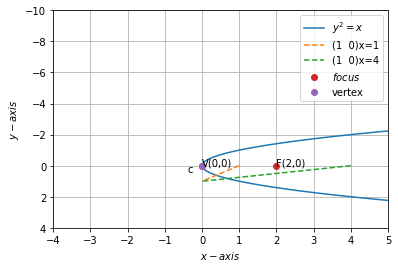
\includegraphics[width=\columnwidth]{download.png}
\caption{Tangent to  parabola in \eqref{eq:parab}  with slope $\frac{1}{5}$. }
\label{fig:parab_tangent}	
\end{figure}



\end{document}
